\chapter{Exercise 3}
\label{chap:3}
This chapter takes a closer look at the AnalysisRunner. Especially some validation is given on why it's assumed that the chosen imlementation works as specified.

\section{Analysis and validation}
To check wheter the chosen implementation works as specified some sanity checks were used.
\begin{itemize}
    \item Validate results for data\_short.dat
    \item Validate results by comparison with other lab participants
    \item Test coverage for Line and Point classes
\end{itemize}

The sanity checks resulted in the assumption that the implementation is correct. All asked lab participants had close results for data\_short and data\_long. The differences might come from JVM optimizations or calculations with double types, which in Java is not 100\% accurate. 

\section{UML class diagrams}
\label{sec:class_diagram}
This section shows the the UML class diagramm for measuring the data in the data\_long.dat file. The whole code can be seen at \ref{sec:appendix_analysisrunner}.

\begin{landscape}
    \begin{figure}
        \begin{center}
            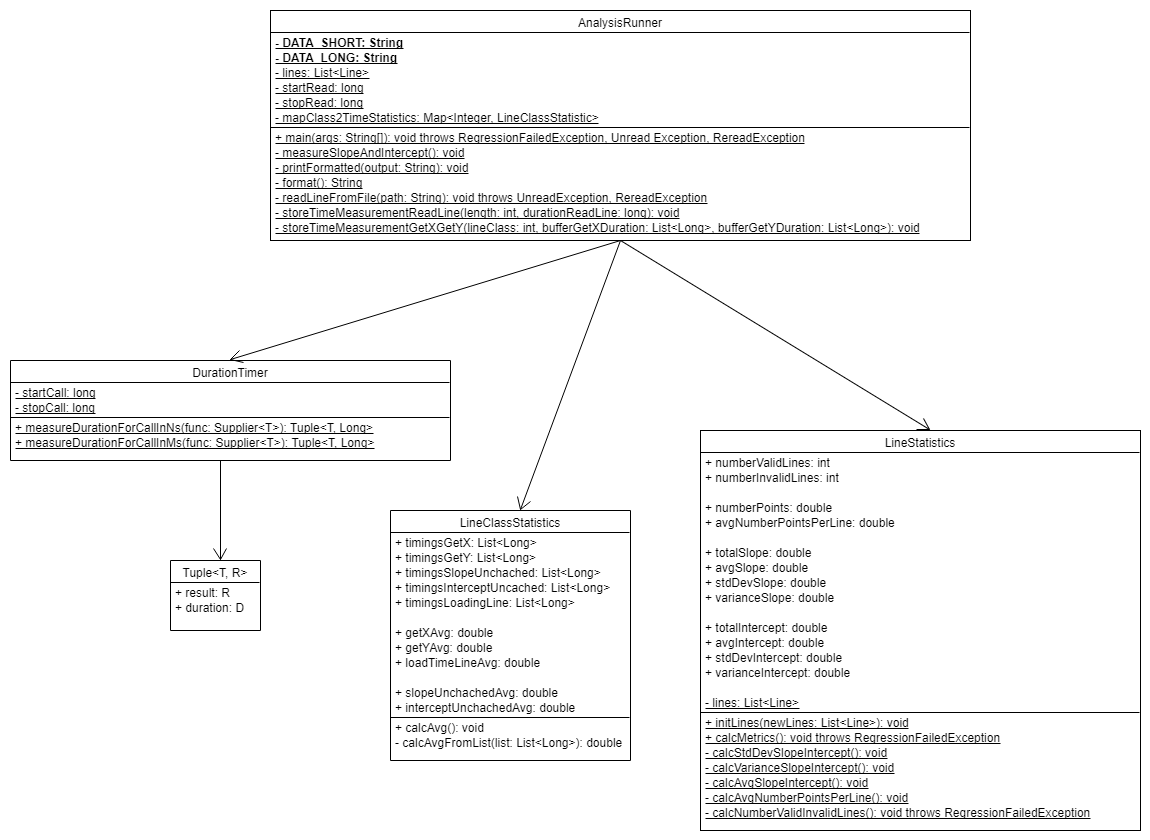
\includegraphics[width=1.60\textwidth]{img/classdiagram.png}
            \caption{UML class diagramm to measure timings}
        \end{center}
    \end{figure}
\end{landscape}

\section{UML sequence diagrams}
\label{sec:seq_diagrams}
In this section UML sequence diagrams are provided for measuring and calculating the wanted statistics. The diagrams are splitted into methods to be more readable. In the end a single UML sequence diagram is provided that references all other provided diagrams. Also for each sequence diagram a small discription is provided and some implementation details are explained.

\subsection{Read lines from file}
This section describes how the provided datafiles are read and the created lines are created. The provided sequence diagram \ref{fig:seq_read} shows how the dataflow is done while reading each line. Firstly, within AnalysisRunner the main method is called, which calls the static method AnalysisRunner.readLinesFromFile(). This creates an object of the provided lineReader class called reader and initializes the path to \lstinline[language=java]{private static final String DATA_LONG}. Then the initialized reader object is used to iterate over the whole data set. This is done via \lstinline[language=java]{reader.nextLine()} which retuns true when there are still lines to read. For each line the reader is used to iterate over every point in the line. For each point the \texttt{getX()} and \texttt{getY()} methods are used to get the X and Y coordinate. This process is timestamped and the duration is calculated. For this \texttt{DurationTimer.measureDurationForCallInMs} is used (see \ref{lst:timerGetX_getY}). This retuns a Tuple with the result of \texttt{getX()} and the time it took to read the data. This data is analysed in \ref{chap:4}

\begin{lstlisting}[language=java, caption=Measure duration for calls getX, label=lst:timerGetX_getY]
    Tuple<Double, Long> timingGetX = DurationTimer.measureDurationForCallInMs(() -> reader.getX());
    //Some Code here
    Tuple<Double, Long> timingGetY = DurationTimer.measureDurationForCallInMs(() -> reader.getY());
\end{lstlisting}

\begin{landscape}
    \begin{figure}
        \begin{center}
            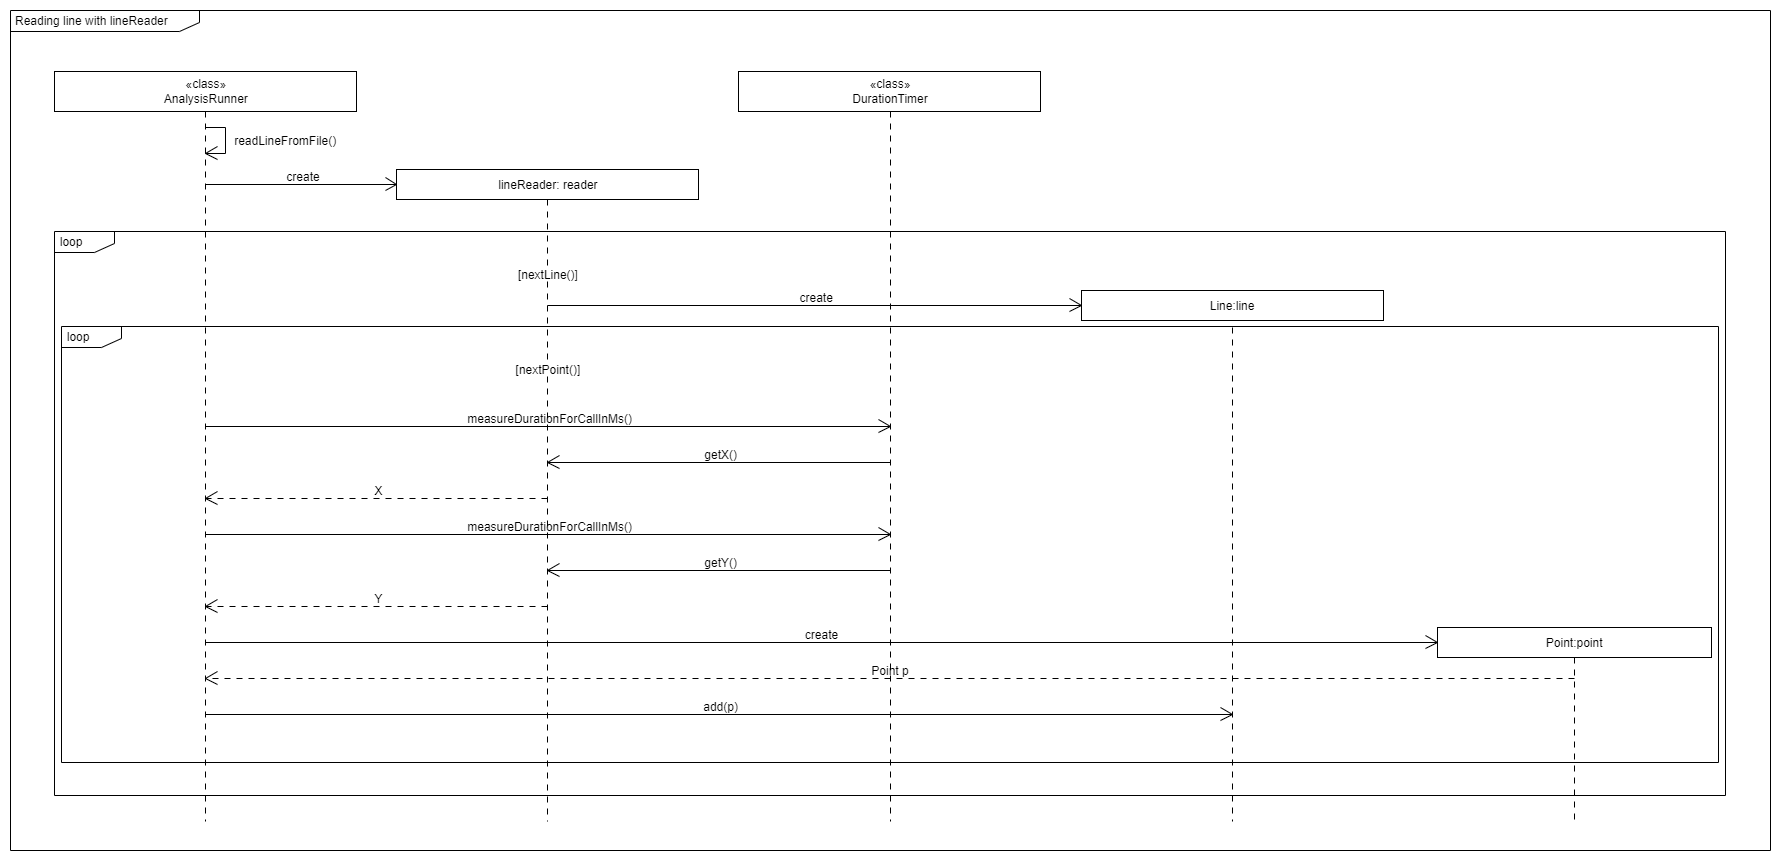
\includegraphics[width=1.75\textwidth, height=0.99\textheight]{img/sequence_read.png}
            \caption{UML sequence diagram for reading in all line in provided data file}
            \label{fig:seq_read}
        \end{center}
    \end{figure}
\end{landscape}

\subsection{Measure slope and intercept}
This method is called before any other method that would calculate slope or intercept, especially \texttt{line.isValid()}, as those methods would calculate slope and intercept and therefore cache the result. To prevent this from happening, slope is also called before intercept else the same problem would occur. The provided sequence diagram \ref{fig:seq_slope_intercept} shows the dataflow and how the DurationTimer is again used to measure the needed time for calculating slope and intercept. It has to be noted, that for measuring the slope and intercept uncached some error handling has to be done in \texttt{DurationTimer.measureDurationForCallInNs()} (see \ref{lst:slope_intercept}).

\begin{lstlisting}[language=java, caption=Error handling in supplier for unchaced slope and intercept, label=lst:slope_intercept]
Tuple<Double, Long> timeSlope = DurationTimer.measureDurationForCallInNs(()-> {
    try {
        return line.slope();
    } catch (RegressionFailedException e) {
        //Happens when line is not valid, as we cannot check without caching slope and intercept
        return Double.NaN;
    }
});
\end{lstlisting}

\begin{landscape}
    \begin{figure}
        \begin{center}
            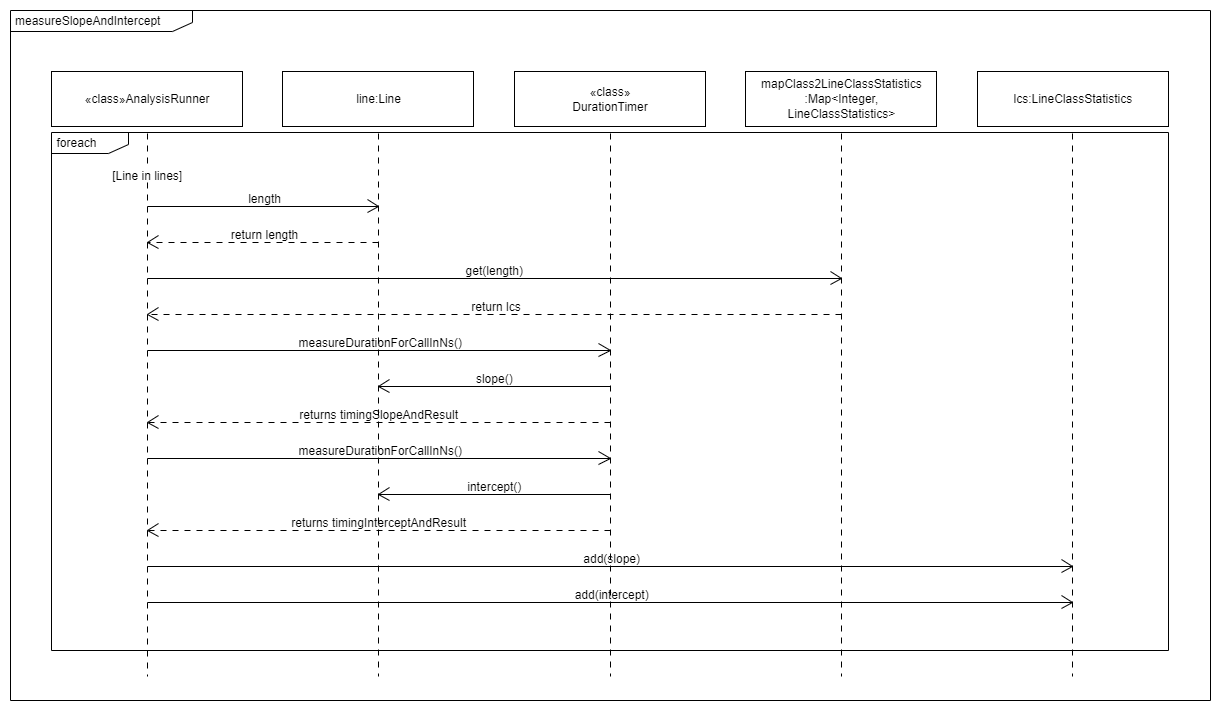
\includegraphics[width=1.75\textwidth, height=0.99\textheight]{img/seq_slope_intercept.png}
            \caption{UML sequence diagram for calculating and measuring time and intercept}
            \label{fig:seq_slope_intercept}
        \end{center}
    \end{figure}
\end{landscape}

\subsection{Calculate averages for line class statistics}
The last sequence diagram shows the calculations of all averages for any line class. All the collected statistics are timeings of some sort they are all stored as lists of long values. The average is calculated with Java streams (see \ref{lst:stream_avgs}).

\begin{lstlisting}[language=java, caption=Java stream used to calculate average of a list, label=lst:stream_avgs]
private double calcAvgFromList(List<Long> list) {
    return list.stream().mapToLong(a -> a).average().orElseGet(() -> Double.NaN);
}
\end{lstlisting}

\begin{landscape}
    \begin{figure}
        \begin{center}
            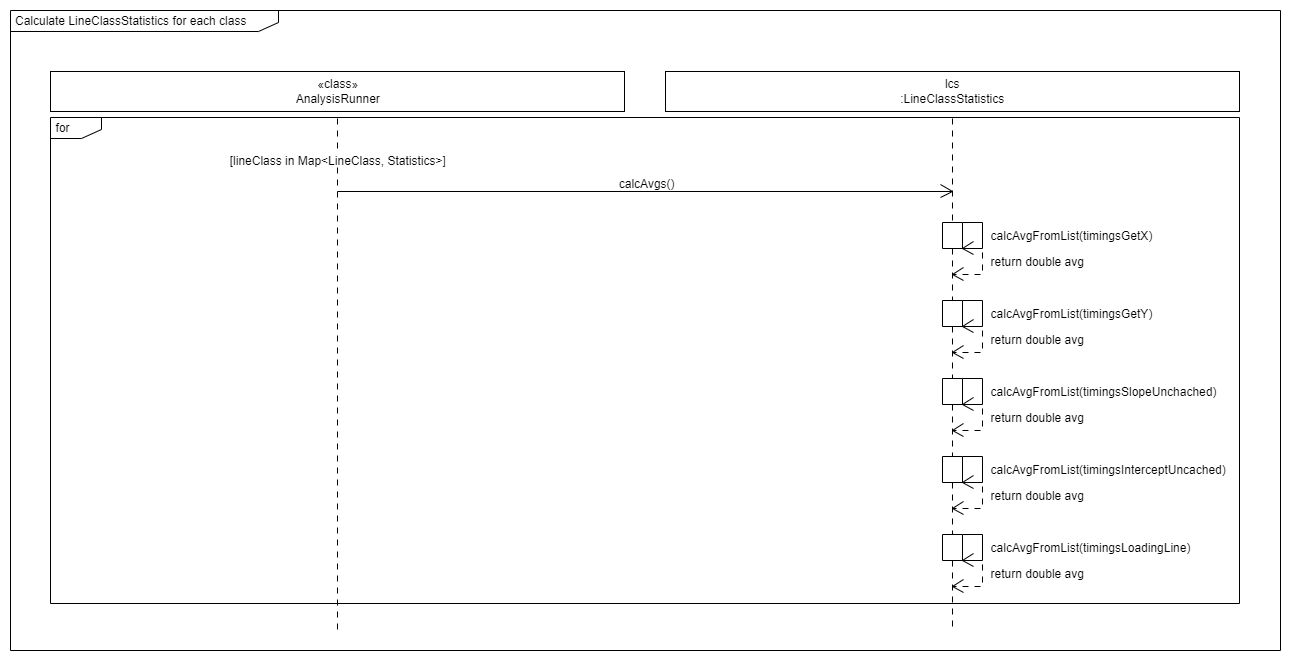
\includegraphics[width=1.75\textwidth, height=0.99\textheight]{img/sequence_lcs_avgs.png}
            \caption{UML sequence diagram describing the calculation of all averages for a line class}
            \label{fig:seq_slope_intercept}
        \end{center}
    \end{figure}
\end{landscape}
